\section{Interactive Technology}\label{2_3_interactiveTechnology}

To build a real time feedback assistance system, a tracking device is needed that supports the slacker in an appropriate way and won't interrupt her. The Microsoft Kinect v2 seems like a suitable tracking system in this context, because the user don't need any further devices to be tracked. But it should be compared with other tracking technologies like the Nintendo Wii, Playstation Move, and motion capture systems, to justify its usage. In the following advantages and drawbacks of these systems will be discussed. Further several studies show how accurate and precise the Microsoft Kinect v2 is, if it can be applied for balancing purposes, give the user appropriate feedback, or useful analysis data for specialist like therapist.

\subsection{Comparison of Tracking Technologies} \label{trackingTechnologie}

The Nintendo Wii consists of a sensor bar with infrared sensors that estimates the position of the Wiimote controller in 3D. Further an accelerometer is integrated in the Wiimote to detect its motion. Thus the user can interact with the console, based on predefined gestures~\cite{Bogdanovych2015-ci, Tanaka2012-ACO}. Gesture recognition is an essential aspect of the slacklining assistance system for giving appropriate feedback regarding the executed exercise. Schlömer et al.~\cite{Schlomer2008-uo} analysed the gesture recognition of the Wii and found an error rate between 5\% and 15\%.

A similar approach with a handheld controller is followed by the PlayStation Move. It contains an RGB camera called Move Eye that is used for tracking the 3D position of a lighting sphere attached on the handheld device named Move wand. The controller contains an accelerometer, gyro sensor and geomagnetic sensor to track the rotation and also support position tracking. In this way more accurate tracking is possible than with the Nintendo Wii~\cite{Bogdanovych2015-ci, Tanaka2012-ACO}.

Both systems are good devices if the controller itself can be replicated as a virtual device like for example in golf or tennis. But they do not track the body movement and the user is bound to her handheld devices to interact with the system. In the slacklining system they could disturb user standing on the slackline. Moreover accurate feedback from the whole body is wanted and thus it should be the actual controlling device. Therefore they seem not to be appropriate devices for the slacklining system.

With a motion capture suit, like \textit{Xsens MVN}~\cite{XsensMvn} or \textit{OptiTrack}~\cite{OptiTrack}, markers have to be attached on the user’s body for tracking her body motion and rotational data. This makes it the best device for high accuracy and precision body tracking. Problems with the suite are that it is very expensive and the setup takes relatively long time because of the marker attachment and the positioning of the tracking cameras. The biggest drawback is the uncomfortable bulky equipment that could interfere the user during the performance~\cite{Bogdanovych2015-ci, Chang2012-hz, Nusman2006-rf}. This makes it an inappropriate device for user tracking on a slackline.

The Microsoft Kinect is a static device that includes a RGB camera and depth sensor. Because the body joints and player position are recognised by these, the user is free in her movement without any further controller. Another advantage is the low price in comparison to the motion control suite, and the low setup time because only the device itself is needed. Problems occur with occlusion of body parts that results in glitches and flawed tracking~\cite{Kajastila2014-ug, Tang2015-wt}. To the user they can be hidden, e.g. by only showing the output of the depth cam~\cite{Holsti2013-kn}. This problem can also occur in the slacklining case because of overlaying feet. Therefore a technical feasibility has to be conducted to show if this is a bigger problem or can be neglected.
%Therefore a feasibility study should be realised to show if this is a bigger problem or can be neglected. 
%The results can be seen in section \textbf{<NUMBER>}. 

With this in mind, the Microsoft Kinect v2 seems like the most suitable device. The recognition of the whole body, freedom of movement, short setup time, and relatively low cost makes it the best system out of the stated devices.

\subsection{Accuracy of the Microsoft Kinect}

In the field of balance training it is necessary to give appropriate feedback for the patient that reveals errors in the performance and support a proper execution. With this in mind user tracking should be good enough to fulfil this criteria. Since Microsoft Kinect is used as the tracking device the accuracy and precision should be assessed.

Lim et al.~\cite{Lim2015-pw} assessed the accuracy of the Kinect with a 3D motion capture system as a reference system. For further understanding please review Figure \ref{fig:bodyWikiAnatomicalTermsOfLocation} regarding expressions to body planes and anatomical directional references. The participants had to execute balance training with complex aperiodic movements in the body planes (Figure \ref{fig:bodyPlanes}). Similar characterization of movements are provided by the Kinect in comparison to the 3D motion capture system. The correlation analysis showed that the Kinect and the 3D motion capture system are highly correlated for the flexion and extensions in the medio-lateral-axis (x-axis) but not on the anterior-posterior-axis (y-axis) and the cranial-caudal-axis (z-axis) (Figure \ref{fig:bodyDirectionalReferences}). This is because the Kinect determine joint locations based on the depth image data and the data input is limited to the depth camera view. Therefore recognition of joint angles in the sagittal and transverse plane is not optimal (Figure \ref{fig:bodyPlanes}). Also the primary goal of the Kinect is to measure the dynamic movements in the coronal (frontal) plane for gaming reasons. It is indeed an effective system to characterize changes in center of mass and movements in the frontal plane during balance training. But it would not be suitable in balance training that require in-depth analyses of joint motions, which is not needed with the slackline assistance.

\begin{figure}[htb]
	\centering
	\begin{minipage}[t]{0.38\linewidth}
		\centering
		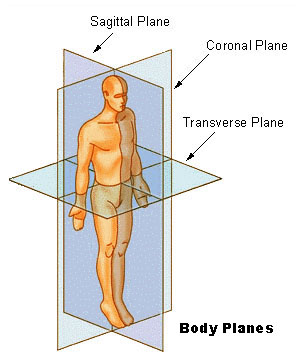
\includegraphics[width=1\linewidth]{Pictures/bodyPlanes}
		\subcaption{Body Planes}
		\label{fig:bodyPlanes}
	\end{minipage}
	\hfill
	\begin{minipage}[t]{0.6\linewidth}
		\centering
		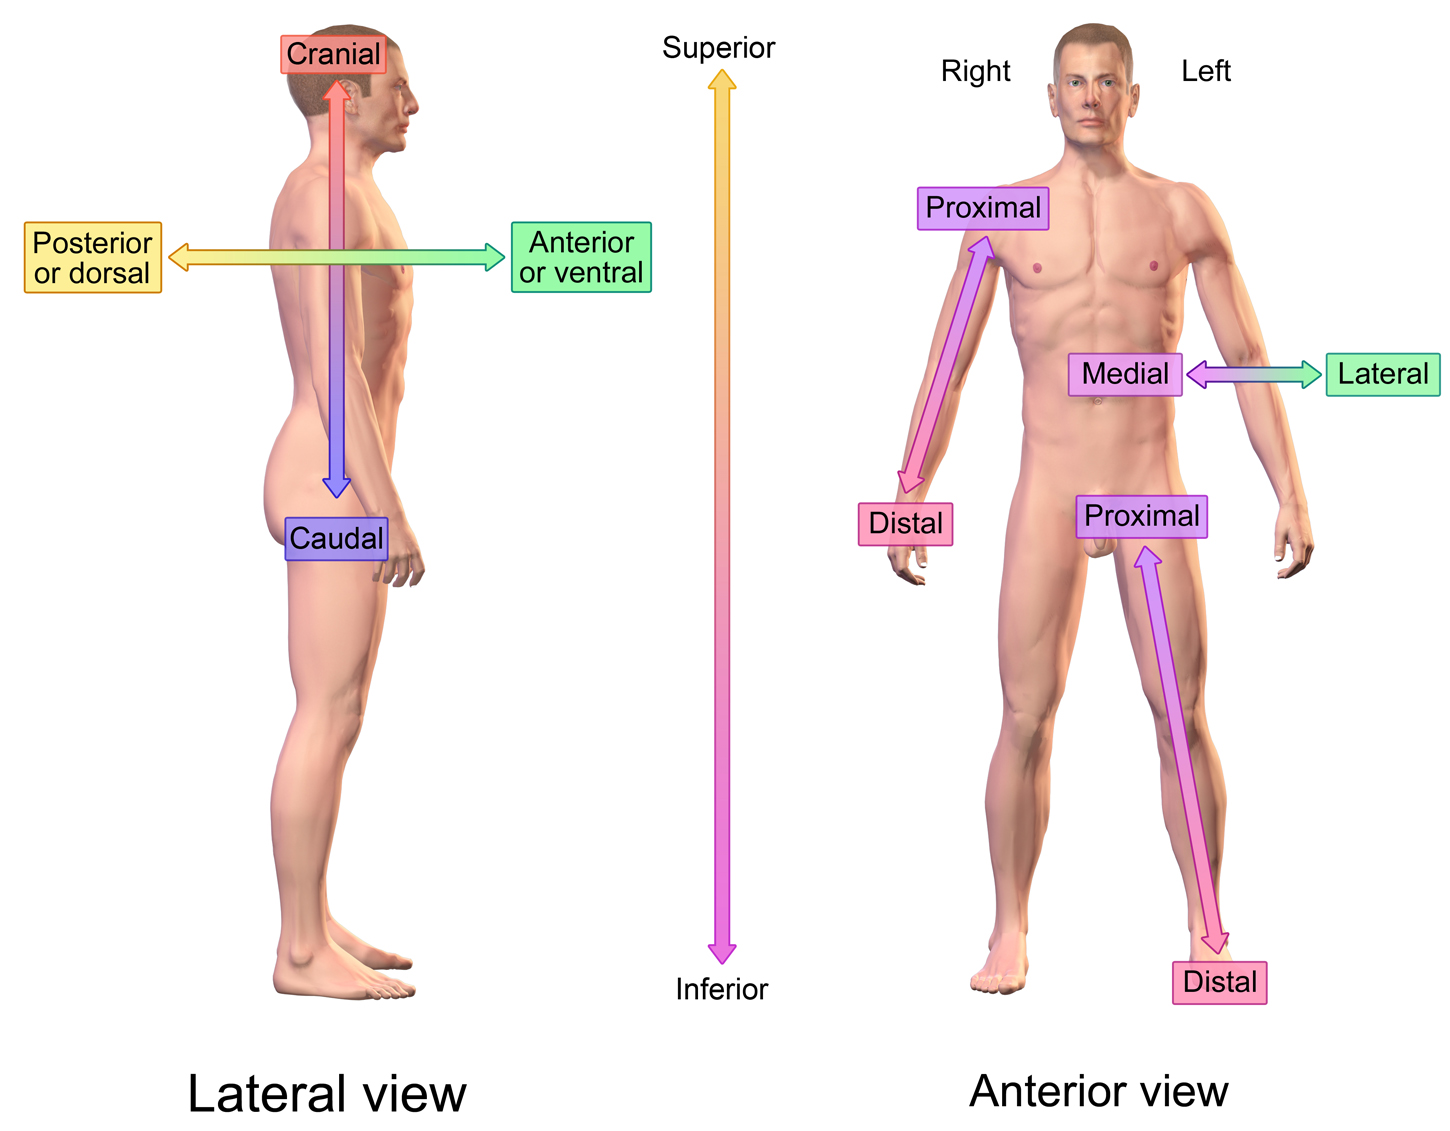
\includegraphics[width=1\linewidth]{Pictures/bodyDirectionalReferences}
		\subcaption{Directional References (modified)}
		\label{fig:bodyDirectionalReferences}
	\end{minipage}
	\caption{Anatomical terms of location~\cite{Wiki2017-ATOL}}
	\label{fig:bodyWikiAnatomicalTermsOfLocation}
\end{figure}

Chang et al.~\cite{Chang2012-hz} focuses mainly on the tracking performance of the Microsoft Kinect as a rehabilitation device in comparison with a high fidelity motion capture system called OptiTrack. In their application the user has to move objects from one side of the screen to the other. Five correct and incorrect movements have been realised and both systems successfully identified them. In trajectory comparison the results of the hand and elbow by the Kinect are very close to the OptiTrack system. Tracking of the shoulder movements are moderate because it involves rotation that the device does not recognizes well. The timing performance comparison shows that the OptiTrack system is negligible faster than the Kinect.

Woolford~\cite{Woolford2015-ub} compared the accuracy and precision of the Kinect v2 with the Qualisys motion capture system for the usage in healthcare applications. He describes that accuracy is the amount of how close a measured quantity to the actual value is. Precision is the similarity of repeated measurements (Figure \ref{fig:systemAccuracyAndPrecisiong}). For example the Kinect skeleton tracking methods are accurate because the average joint position data is very close to the actual physical position. Regarding his definition of precision, the joint position data is not always precise because the data spreads in its position of the frame. The results show that the Kinect V2 is accurate but imprecise for body parts whose center of mass cannot be easily identified like the shoulder. For smaller body parts as well as between two body parts such as elbow or wrist the accuracy and precision is very high. 

\begin{figure}[htb]
	\centering
	\begin{minipage}[t]{0.49\linewidth}
		\centering
		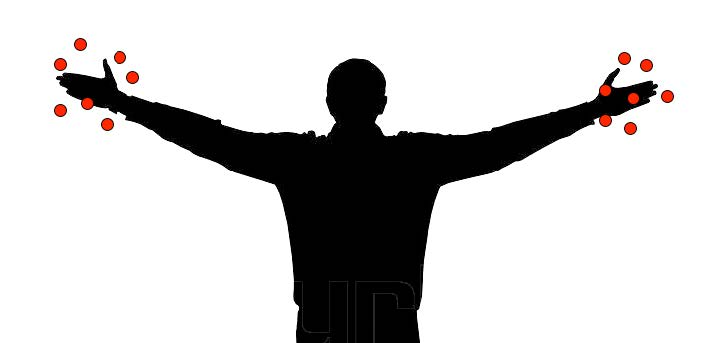
\includegraphics[width=1\linewidth]{Pictures/systemInaccurateImprecise}
		\subcaption{Inaccurate and imprecise system generates random-like measurements}
		\label{fig:systemInaccurateImprecise}
	\end{minipage}
	\hfill
	\begin{minipage}[t]{0.49\linewidth}
		\centering
		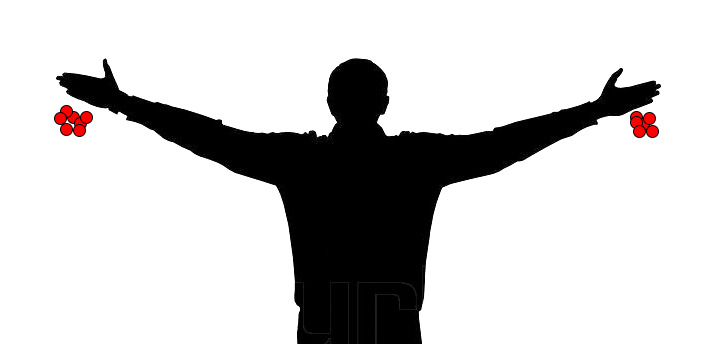
\includegraphics[width=1\linewidth]{Pictures/systemInaccuratePrecise}
		\subcaption{Inaccurate but precise system, where measurements are close to each other but have systematic error}
		\label{fig:systemInaccuratePrecise}
	\end{minipage}
	\hfill
	\begin{minipage}[t]{0.49\linewidth}
		\centering
		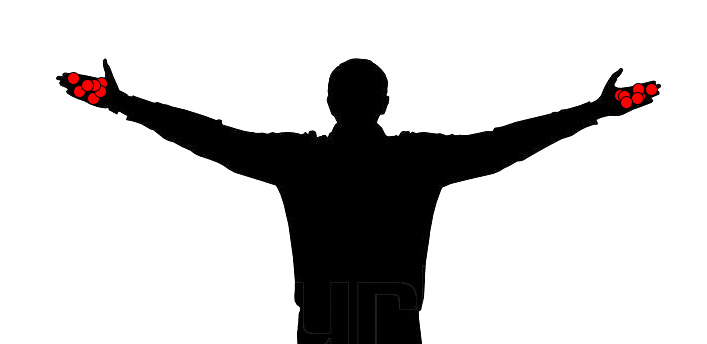
\includegraphics[width=1\linewidth]{Pictures/systemAccuratePrecise}
		\subcaption{Accurate and precise system generates measurements that are close to the real world}
		\label{fig:systemAccuratePrecise}
	\end{minipage}
	\hfill
	\begin{minipage}[t]{0.49\linewidth}
		\centering
		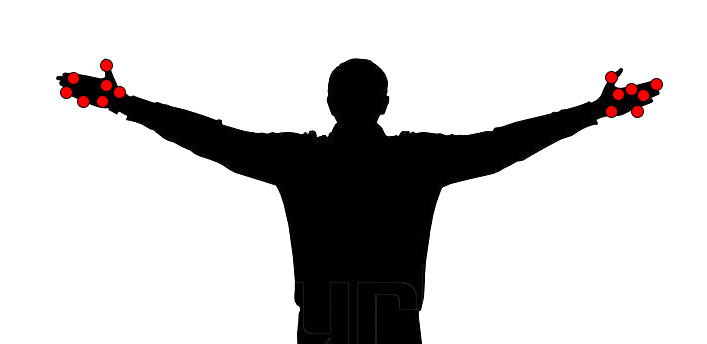
\includegraphics[width=1\linewidth]{Pictures/systemAccurateImprecise}
		\subcaption{Accurate and suffice precise system generates measurements that are close to each other and are not systematically biased}
		\label{fig:systemAccurateImprecise}
	\end{minipage}
	\caption{Definition of accuracy and precision~\cite{Woolford2015-ub}}
	\label{fig:systemAccuracyAndPrecisiong}
\end{figure}

The Microsoft Kinect v2 can indeed be compared with high performance tracking devices. If no detailed analysis is needed, it provides reliable and appropriate data. For the assistance system it should provide sufficient data to track the user and give useful feedback

\subsection{Implementation in Balance Training Scenarios}

Like already stated Chang et al.~\cite{Chang2012-hz} not only assessed the accuracy of the Microsoft Kinect but also if it could fit as an alternative training device in rehabilitation training. The results show that it provides enough usable feedback to the therapists to be an appropriate device for medical uses. Woolford~\cite{Woolford2015-ub} state that the Microsoft kinect is a useful device for monitoring such exercises. The set-up is relatively easy and the tracking is appropriate for exercises in a healthcare environment. Lim et al.~\cite{Lim2015-pw} investigated the usage of Microsoft Kinect in the field of falling risk. They tracked characterizing movements and found that it is an useful device for balance training. Ustinova et al.~\cite{Ustinova2014-ml} used the Kinect to improve the postural control as well as coordination deficits from chronic traumatic brain injury patients. It resulted in improvements of postural stability, movement performance and motoric coordination. The participants were also very satisfied whereas normal exercises have been stated as boring. Pisan et al.~\cite{Pisan2013-sf} used the device to investigate the prediction of the loss of balance for elderly users with a step training program. The user preferred doing exercises with the system and the tests matched also the expectation of the researcher. An integration in promoting the postural control for parkinson disease with 

Kinect games were elaborated by Pompeu et al.~\cite{Pompeu2014-yl, Pompeu2015-vp}. The results affirm that the patients improve in balance purposes and motoric movements with this help.

Furthermore Estapa et al.~\cite{Estepa2016-oj} and Freitas et al.~\cite{Freitas2012-ae} collected data of execution from patients for medical reviews. Both developed a motor rehabilitation game. It is used to support therapeutic exercises and evaluate biomechanics of the patients. This allows subsequent analysis of the performance data for the therapist.

This approach of data analysis was also integrated by Garrido et al.~\cite{Garrido2013-zs} but in addition they elaborate if the Kinect can serve as a rehabilitation home assistance. Many patients are thrown out of their daily life environment for accessing traditional rehabilitation training in a medical center. Here the patient incorporate the system into their daily life and avoid such trips. The medical stuff gets all relevant parameters due to the transmission of the recordings from the exercises to the medical center. Beside this they get more time because nobody has to observe the training.

Keeping the stated results in mind shows that the Microsoft Kinect is a promising system for balance exercises that provides sufficient accurate and usable feedback. It can be embedded in a variation of fields as rehabilitation system, home assistance, or preventative technique. The aspect to motivate patients with an exergame approach and enjoyable user interface can also lead to successful exercise execution, which is part of the next section.